\chapter{Classification and Prediction}

Thus far in the book, the term \emph{information}
has been used sparingly and when
it has been used, we have purposely been imprecise as to its meaning.
Although, everyone  has an intuitive feeling for what information is,
it is difficult to attach
a meaningful quantitative definition to the term. In the context of
communication systems, Claude Shannon was able to do exactly this,
and as a result, opened up an entirely new view of communication systems
analysis and design \cite[p.~123]{Albano1991}.
The principal contribution of Shannon's information theory to date has been
to allow communication theorists to establish absolute
bounds on communication systems performance that cannot be exceeded no matter
how ingeniously designed or complex our communication systems are.
Fundamental physical limitations on communication systems performance is
another topic that has been largely ignored in the preceding chapters,
but it is a subject of exceptional practical importance.
For example, for any of the numerous communication systems developed
thus far in the book, we could decide to design
a new system that would outperform the accepted standard for a particular
application. The first question that we should ask is: how close is the
present system to achieving theoretically optimum performance?
If the existing communication system operates at or near the fundamental
physical limit on performance, our task may be difficult or impossible.
However, if the existing system is far away from the absolute
performance bound, this might be an area for fruitful work.

\section{What is Classification? What is Prediction?}
\label{ch01.sec11.1}

Of course, in specifying the particular communication system under
investigation, we must know the important physical parameters,
such as transmitted
power, bandwidth, type(s) of noise present, and so on,
and information theory allows these constraints to be incorporated.
However, information theory does not provide a way for communication system
complexity to be explicitly included.
Although, this is something of a drawback, information theory itself provides
a way around this difficulty, since it is generally true that as we approach
the fundamental limit on the performance of a communication system,
the system complexity increases, sometimes quite drastically.
Therefore, for a simple communication system operating far
from its performance bound, we may be able to improve the performance
with a relatively modest increase in complexity.
On the other hand, if we have a rather complicated communication system
operating near its fundamental limit, any performance improvement may
be possible only with an extremely complicated system.

In this chapter we are concerned with the rather general block diagram
shown in Figure~\ref{ch01.fig11.1.1}. Most of the early work by
Shannon and others ignored the source  encoder/decoder blocks and
concentrated  on bounding the performance of the channel
encoder/decoder pair. Subsequently, the source  encoder/decoder blocks
have attracted much research attention.  In this chapter we consider
both topics and expose the reader to the nomenclature used in the
information theory literature.
Quantitative definitions of information are presented in
Sec.~\ref{ch01.sec11.2} that lay the foundation for the remaining
sections. In Secs.~\ref{ch01.sec11.2} and~\ref{ch01.sec11.2} we present
the fundamental source and channel coding theorems, give some examples,
and state the implications of these theorems.
Section~\ref{ch01.sec11.2} contains a brief development of rate
distortion theory,
which is the mathematical basis for data compression.
A few applications of the theory in this chapter are presented
in Sec.~\ref{ch01.sec11.2}, and a technique for variable-length
source coding is given in Sec.~\ref{ch01.sec11.2}.
\begin{equation}
x = a + b - \sqrt{q}
\end{equation}
Of course, in specifying the particular communication system under
investigation, we must know the important physical parameters,
such as transmitted
power, bandwidth, type(s) of noise present, and so on,
and information theory allows these constraints to be incorporated.
However, information theory does not provide a way for communication system
complexity to be explicitly included.
Although, this is something of a drawback, information theory itself provides
a way around this difficulty, since it is generally true that as we approach
the fundamental limit on the performance of a communication system,
the system complexity increases, sometimes quite drastically.
Therefore, for a simple communication system operating far
from its performance bound, we may be able to improve the performance
with a relatively modest increase in complexity.
On the other hand, if we have a rather complicated communication system
operating near its fundamental limit, any performance improvement may
be possible only with an extremely complicated system.

\subsection{And Yet More of the Same}

\noindent In this chapter we are concerned with the rather general block diagram
shown in Figure~\ref{ch01.fig11.1.1}. Most of the early work by
Shannon and others ignored the source  encoder/decoder blocks and
concentrated  on bounding the performance of the channel
encoder/decoder pair. Subsequently, the source  encoder/decoder blocks
have attracted much research attention.  In this chapter we consider
both topics and expose the reader to the nomenclature used in the
information theory literature.
Quantitative definitions of information are presented in
Sec.~\ref{ch01.sec11.2} that lay the foundation for the remaining
sections. In Secs.~\ref{ch01.sec11.2} and~\ref{ch01.sec11.2} we present
the fundamental source and channel coding theorems, give some examples,
and state the implications of these theorems.
Section~\ref{ch01.sec11.2} contains a brief development of rate
distortion theory,
which is the mathematical basis for data compression.
A few applications of the theory in this chapter are presented
in Sec.~\ref{ch01.sec11.2}, and a technique for variable-length
source coding is given in Sec.~\ref{ch01.sec11.2}.
\begin{itemize}
\item This is a bullet list with a short item.
\item And another item that is much longer so that we can make sure it is
formatted correctly and so forth and so on.
\item And a final short item.
\end{itemize}

\begin{figure}
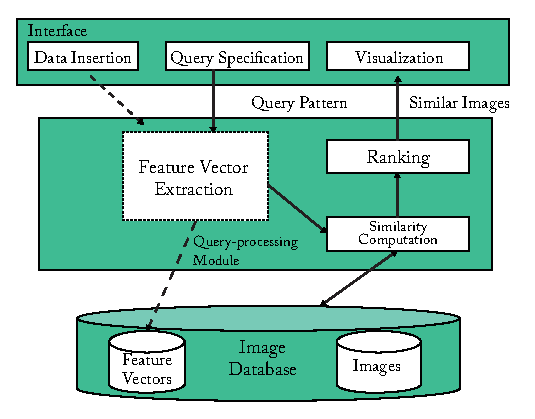
\includegraphics[width=24pc]{sample-figure}
\caption{This is a caption for this figure. It is fairly long so we can make
sure it looks good when occupying more than one line. Here is one more
sentence to make it longer.}
\label{ch01.fig11.1.1}
\label{fig:query-specification}
\end{figure}

In this chapter we are concerned with the rather general block diagram
shown in Figure~\ref{ch01.fig11.1.1}. Most of the early work by
Shannon and others ignored the source  encoder/decoder blocks and
concentrated  on bounding the performance of the channel
encoder/decoder pair. Subsequently, the source  encoder/decoder blocks
have attracted much research attention.  In this chapter we consider
both topics and expose the reader to the nomenclature used in the
information theory literature.
\begin{align}
a& = b + c\\
x&= \frac{1}{2} a
\end{align}
Quantitative definitions of information are presented in
Sec.~\ref{ch01.sec11.2} that lay the foundation for the remaining
sections. In Secs.~\ref{ch01.sec11.2} and~\ref{ch01.sec11.2} we present
the fundamental source and channel coding theorems, give some examples,
and state the implications of these theorems.
Section~\ref{ch01.sec11.1} contains a brief development of rate
distortion theory,
which is the mathematical basis for data compression.
A few applications of the theory in this chapter are presented
in Sec.~\ref{ch01.sec11.2}, and a technique for variable-length
source coding is given in Sec.~\ref{ch01.sec11.2}.

Only the binary Huffman procedure has been described here,
but nonbinary codes can be designed using the Huffman method.
The details are somewhat more complicated and nonbinary codes
are less commonly encountered than binary ones,
so further discussion is left to the problems and the literature.

\section{Case Study}
\label{sec:case-study}

In this section, we exemplify how the 5S extensions for content-based image retrieval can be explored to define an image search service in the context of the CTRnet project.
The Crisis, Tragedy, and Recovery Network (CTRnet)~\cite{Balzer2007} objectives include to develop better
approaches toward making technology useful for archiving information about such events, and to support
analysis of rescue, relief, and recovery, from a digital library  perspective. CTRnet has
several modules, including crawling, filtering, a Facebook application, visualization, metadata
search, and Content-Based Image Retrieval (CBIR). 

The CBIR module
builds upon the EVA tool for evaluating image descriptors for content-based image retrieval \cite{Bierman2005}. Eva integrates the most common stages of an image retrieval process and provides functionalities to facilitate the comparison of image descriptors in the context of content-based image retrieval.

In this case study, we consider the scenario in which a user is interested in finding images in the CTRnet collection that are similar to a particular photo provided as example. The objective is to identify images that could be used in a report on damages caused by an earthquake. 
In this example, the query specification $q$ would be a tuple $q = (H_q, Contents_q, P_q)$, where $q$ is an image (see Figure~\ref{fig:query-specification})
 Thus, $q =
((V_q, E_q), L_q, F_q), Contents_q, P_q)$, where $V_q = {v_1}$; $E_q =\emptyset$; $L_q={' Cathedral\_P\_A\_P.jpg'}$; $F_q: V_q\cup E_q
\rightarrow L_q$, $Contents_q$ is the stream of the query image; and $P_q: V_q
\rightarrow Contents_q$.

\begin{table}
\caption{This is a little table here.}
\label{tab:coordinates}
\begin{tabular}{ccccc}
\hline
Foo& Bar& Zoo& Snork& Quux\\
\hline
 0 & 0 & 1 & 2 & 4\\
 0 & 0 & 3 & 2 & 4\\
 3 & 3 & 1 & 0 & 1\\
 3 & 1 & 4 & 2 & 1\\
 3 & 4 & 4 & 2 & 2\\
\end{tabular}
\end{table}

In this chapter we are concerned with the rather general block diagram
shown in Figure~\ref{ch01.fig11.1.1}. Most of the early work by
Shannon and others ignored the source  encoder/decoder blocks and
concentrated  on bounding the performance of the channel
encoder/decoder pair. Subsequently, the source  encoder/decoder blocks
have attracted much research attention.  In this chapter we consider
both topics and expose the reader to the nomenclature used in the
information theory literature.

\section{Entropy and Average Mutual Information}
\label{ch01.sec11.2}

Consider a discrete random variable $U$ that takes on
the values $\{u_1, u_2, \dots, u_M\}$, where the set of possible
values of $U$ is often called the \textit{alphabet} and the elements
of the set are called \textit{letters} of the alphabet. Let $P_U(u)$
denote the probability  assignment  over the alphabet, then we can
define the \textit{self-information} of the event $ u = u_j $ by
\begin{equation}
  I_U \left( u_j \right) = \log \frac{1}{P_U (u_j)} = - \log P_U
    \left( u_j \right)~.
\label{ch01.eq11.2.1}
\end{equation}
The quantity $I_U (u_j) $ is a measure  of the information  contained
in the event $ u = u_j$. Note that the base of the logarithm in
Eq.~\eqref{ch01.eq11.2.1} is unspecified. It is common
to use base $e$, in which case $I_U (\cdot) $ is in natural units (nats),
or base 2,  in which case $I_U(\cdot)$ is in binary units (bits).
Either base is acceptable since the difference in the two bases is just a
scaling operation. We will use base 2 in all of our work,
and hence $I_U(\cdot)$ and related quantities will be in bits.
The average or expected value of the self-information is called the
\textit{entropy,} also discrete entropy or absolute entropy, and is given by
\begin{equation}
 \displaystyle H(U) = - \sum^M_{j=1} P_U \left(u_j\right)
    \log P_U \left(u_j \right)~.
\label{ch01.eq11.2.2}
\end{equation}
The following example illustrates the calculation of entropy and how it is
affected by probability assignments.

\section{Exercises and Projects} 
\label{cbir:exercises}

\begin{enumerate}
\item
How might CBIR be applied so teachers with a computer and connected camera can be reminded of the names of students in their class?

\item Consider the two colourful images (Image A and Image B) showed below, represented in the RGB color space. Suppose that the intensity values of each pixel in all bands (R, G, and B) are the same. Furthermore, each $(R,G,B)$ triplet is represented by a single intensity value. For example the triplet $(R,G,B)= (2,2,2)$ is represented by the intensity value $2$.

Suppose also that the colour space was quantized in five colors with intensity values 0, 1, 2, 3, and 4.

\item Compute the $L_1$ between the {\em Color Histograms} (5
  bins) of the two images. The $L_1$ distance between two color histograms $H_A$ and $H_B$ is computed as follows: $L_1(H_A, H_B) = \sum_{i=1}^{K}|H_A[i]- H_B[i]|$, where $K$ is the size of both histograms (5, in the case).


\item By considering both the feature vector extraction function and the distance function defined of the descriptor {\em Color Coherence Vector -- CCV}~\cite{Burns2006}, compute the distance
  $\delta_{CCV}(A,B)$ between the two images.

\item Consider the existence of two classes ({\em class 1} and {\em
class 2}) composed of five images each. Consider the existence of three different descriptors ({\em descriptor 1}, {\em descriptor 2}, and {\em descriptor 3}), whose feature vector extraction functions extract vectors belonging to the $R^2$ space. 
Table~\ref{tab:coordinates} shows the coordinate of each image of each class, considering the three descriptors.
\end{enumerate}

